% -*- fill-column: 85; -*-
%!TEX root = ../dissertation.tex
\section{Design}
\label{s:design}

\begin{figure}[t!]
	\centering
	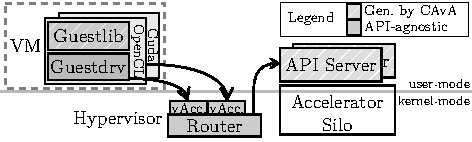
\includegraphics[width=0.8\textwidth]{ava/images/design_high_level.pdf}
	\caption{Overview of \hirafull. Components with striped backgrounds are API-specific and are generated from an API specification. Components with solid backgrounds are API-agnostic and only need to be implemented once per hypervisor (or per hypervisor-OS combination.}
	\label{fig:design}
\end{figure}

The resulting novel design, \emph{\hirafull (\hira)} is shown in
Figure~\ref{fig:design}. Applications in the guest VM link against a custom
``Guestlib'' which is a drop-in replacement for the API the application uses
(e.g., OpenCL, CUDA). The ``guestlib'' traps API calls (\emph{the interposition
mechanism}) and serializes their parameters and any relevant environment
information to a buffer that is exposed to it by a custom driver (shown as
``Guestdrv'' in the figure). A single ``guestdrv'' driver is reusable across
all API frameworks in the guest (the same driver can be loaded for each API
for improved security), and importantly only one driver needs to be
implemented for a given OS-hypervisor combination. This driver interfaces with
the ``vAcc'' virtual accelerator that the hypervisor presents guest VMs with.
The ``vAcc'' is an abstract virtual device that exposes the typical hardware
interface (MMIO Base Address Registers, Command Queues, etc.), and is used as
\emph{the source endpoint} for routing communication through the hypervisor.
Importantly this virtual device is \emph{not a virtual accelerator} in that it
isn't specialized to any one DSA. Like the ``guestdrv'' driver, only a single
implementation of this virtual device is necessary per hypervisor. The virtual
accelerator acts as \emph{the destination endpoint} of the hypervisor managed
transport for interposed API calls. The method used to communicate between the
guestdriver and the virtual accelerator is considered the \emph{interposition
transport}: this could be a FIFO backed by shared memory, or a network based
transport (TCP/IP). All serialized API calls received by the ``vAcc'' are then
processed by, a hypervisor module (``Router'' in the Figure) that enforces
resource control and scheduling policies at the granularity of the API calls.
Semantic information about the interposed API function is captured in the API
specification written in \lapis. The API calls are then forwarded to a per-VM
``API server'' that executes the API call on the vendor's API framework
(``Accelerator Silo'' in the figure) in the host. Results of the API
invocation are captured, serialized, and transported back to the guest application from the host.

Using hypervisor-managed transport recovers interposition, but also complicates
compatibility and introduces engineering effort: \hira requires custom guest
libraries, guest drivers, and API servers for each OS and API, and
API-specific resource-management code in the hypervisor (policy code for the
``Router''). Our prototype implementation, \AvA, mitigates this with automated
construction (\S\ref{s:api}). Automatically generating code to implement \hira
components presents several challenges which follow from the need to specify
API semantics and policies for which existing Interface Description Languages
(IDLs)~\cite{Lamb1987,MSIDL} are not applicable. \AvA uses a DSL called \Lapis,
a compiler called \CAvA, and device-agnostic transport components to address
these challenges.

\AvA targets \emph{compute offload} accelerator APIs, such as OpenCL, CUDA,
and TensorFlow, which control an accelerator explicitly through data transfer
and task creation interfaces. \AvA consists of API-agnostic para-virtual stack
components to implement transport and dispatch for API remoting, API-specific
components that interpose and execute the API functions, and a compiler---%
\CAvA, which generates the API-specific components from a specification of the
API. The API specification is written in a new high-level specification
language, \Lapis, that is used to both capture both the syntax and semantics
of the API. The ``Router'' may be deployed in the hypervisor or in an
appliance VM to support type I and II hypervisors~\cite{popek-goldberg}.

\section{\AvA Components}

\begin{figure*}[t]
    \centering
    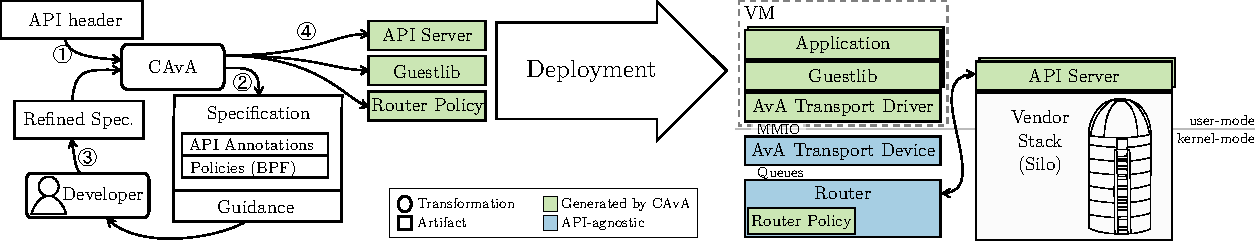
\includegraphics[width=\textwidth]{ava/images/overview.pdf}
    \caption{Overview of \AvA.}
    \label{fig:overview}
    \vspace*{-1em}
\end{figure*}

Figure~\ref{fig:overview} provides an overview of the interaction between the
various components in a \AvA-generated design, and the work-flow to support a
new API with \AvA (\S\ref{sub:workflow}) and the \AvA stack.

The \parname{guest library} is generated by \CAvA from the \Lapis
specification. It provides the same symbols as the vendor library for the
application to link against. The guest library intercepts all API functions
called by guest applications, marshals function arguments and implicit
state, and forwards the call through the transport channel for remote
execution.

The \parname{guest driver} interacts with the \vdev exposed to the
VM and provides a transport channel endpoint in the VM. Each guest-driver
manages a set of command queues that are used to forward API calls to the
\worker via the router. \CAvA generates a separate transport driver instance
for each API framework to preserve cross-framework isolation and guest OS
interposition.

The \parname{\vdev} is an abstract device exposed to the guest to
forward API calls between the guest and the \worker. The \vdev exposes MMIO
BARs for control (Our implementation uses 4 BAR registers: one stores vm\_id,
one stores the physical address of a buffer used to implement zero-copy, one
to notify KVM when the guestdrv is installed, and the last to notify KVM when
an app is spawned.) and a command queue interface. It is API-agnostic, and its
purpose is to provide an interposable interface for the hypervisor.

The \parname{router} is an API-agnostic extension to the hypervisor
that implements \AvA's interposition logic. The router performs security
checks and enforces scheduling policies on forwarded API calls according
to the \Lapis specification.

The \parname{\worker} is an API-specific user-space process
generated by \CAvA. It runs either in an appliance VM (with PCIe pass-through
access to the physical device) or in the host. The \worker executes forwarded
calls on behalf of the guest application. A given \Worker is dedicated to a
single guest process, leveraging process-level isolation when the hardware
supports it to guarantee fault and device context isolation.

The router, the \worker, and vendor device drivers are considered part of the
Trusted Computing Base, while the guest library and the guest \vdev driver are
untrusted. The router may rely on the \worker to provide semantic information
that may be specific to a given API, e.g., the \worker may provide device
resource accounting information to the router for resource management.

\section{Developer Work-flow}
\label{sub:workflow}

\AvA's API-agnostic components must be implemented for each hypervisor, along
with the guest drivers needed for each supported guest OS. The development
effort to build them is amortized across all of the accelerators and framework
APIs supported.

\AvA's API-specific components are generated from \Lapis by \CAvA to
plug into \AvA's API-agnostic components. \Lapis (\S\ref{s:api}) is used to
annotate the functions in an API and provide an overview of how the API
controls accelerator resources. This semantic information enables automatic
construction of the API remoting system.

Figure~\ref{fig:overview} shows the work-flow to support a new API with \AvA.
First, \CAvA automatically generates a preliminary \Lapis specification from
the unmodified API header file. The programmer refines the specification with
guidance from \CAvA; adding information missing from the header file, e.g.,
buffer sizes or implicitly referenced state. Once the developer is satisfied
with the API specification, she invokes \CAvA to generate code for the
API-specific components and the customized driver. \CAvA also generates
deployment scripts. When a new version of an API is released, the same process
can be used, starting with the previous specification.

\subsection{Communication Transport}
\label{s:design_transport}

\AvA relies on an abstract communication channel that defines how interposed
API calls and their associated data buffers are sent to the host, and results
are sent back, validated, and received. The channel provides an interposition
point to track resources and invoke control policies. Using an abstract
interface allows hypervisor developers to choose the best available
communication transport (e.g., shared memory FIFOs vs RDMA). While the channel
explicitly requires that all communication between the guest and the \worker
must take place through the router, no assumptions are made about the actual
location of components, which may be disaggregated.
The transport handles two types of payloads: \emph{commands} which contain
opaque arguments and metadata for calls (e.g., thread ID and function ID) and
\emph{data} which contains buffers referenced from the arguments (e.g., bulk
data). As communication is bidirectional in a virtualization system, \AvA also
provides support for function callbacks from the \worker to the guest library.
Callbacks are fundamental in many frameworks, e.g., TensorFlow, and must be
run in the guest VM.

\subsection{Sharing and Protection}
\label{s:protection}

\AvA re-purposes process-level isolation mechanisms (e.g. memory protection)
provided by the accelerator silo (when available) to simplify supporting
cross-guest isolation. We anticipate that emerging accelerators will support
process-level isolation, as all GPUs do today. While the lack of hardware
virtualization support represents an obstacle for accelerator virtualization.
DSA stack structure is just as important. Even if all accelerators were to
support process-level virtualization in hardware, a software based
API-remoting scheme like \AvA will still be necessary unless vendor stacks
expose the interfaces required to take advantage of that support.

For accelerators that do not natively support process-level isolation,
\AvA can still share the device: semantic information from additional \Lapis
descriptors enable us to generate code that supports coarse-grain
time-sharing. Metadata on the API functions that create and destroy
connections to the hardware allows the \CAvA to insert additional logic in the
device open/close calls to transparently spin until the device becomes
available. This solution admits no concurrency between tenants, but enables
protected sharing for devices which cannot otherwise be shared.

\subsection{Scheduling and Resource Allocation}
\label{s:rate_limit}
\label{s:api_throttling}

\AvA can enforce policies (e.g., rate limiting) on shared resources, e.g.,
device execution time, by tracking resource consumption and invoking policy
callbacks that change how API calls from guests are scheduled. We envision the
virtualization developer providing these policy callbacks in the \Lapis
specification, and using annotations on the functions of the APIs to identify
how resources are consumed. When such an annotation is unavailable, \AvA falls
back to coarse-grained estimation of resource utilization, for example, using
wall-clock time to approximate device execution time.

\subsection{Memory Management}
To support memory sharing on devices with onboard memory, \Lapis resource
usage annotations on the functions of an API enable generated code to track
the device memory allocated to each guest VM. Resource accounting code is
auto-generated from semantic knowledge of the device memory allocation APIs
provided by annotations in the API specification (e.g., memory types and how
to compute size of buffer). This enables the hypervisor to enforce policies at
the granularity of API function calls. For example, If a device memory
allocation request would exceed the guest's quota, the hypervisor instructs
the \worker to return the appropriate Out-of-Memory (OOM) error for the
allocation request.